% APPLICAZIONI REALI
\section{Applicazioni reali}
I grafici che seguono rappresentano i modelli tariffari scelti dalle varie piattaforme e mostrano il loro comportamento al variare del ``carico di lavoro''.
Nell'asse delle ascisse si trova il numero di immagini (numero di chiamate con un'immagine ogni chiamata) processate al mese,
mentre l'asse delle ordinate il corrispondente costo in dollari americani\footnote{Regione: West US}.
E' stata scelta questa valuta poiché tutti i servizi coprono il territorio americano (almeno in parte), mentre non è così per altre zone come l'europa;
una valuta come il dollaro, quindi, offre un metro di paragone fra tutti i servizi.

Il primo grafico in \ref{grafico-1} mostra le differenze di prezzo per riconoscimento di oggetti con un basso carico di immagini, includendo anche i piani gratuiti.
Come si può notare per poche immagini il sevizio offerto da Google non è conveniente, infatti offre gratuitamente solo 1000 chiamate al mese. 
Bisogna però ricordare che l'IBM Visual Recognition offre mensilmente il maggior numero di chiamate ma il conteggio è giornaliero. 
\begin{figure}[htbp]
\begin{center}
	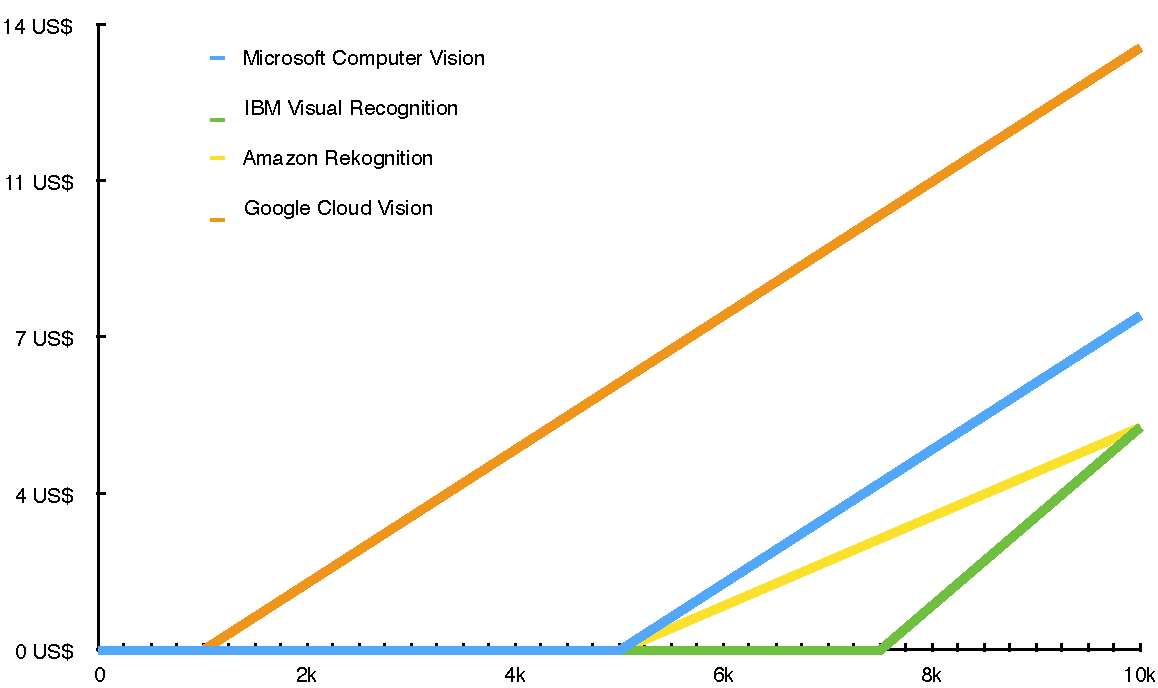
\includegraphics[scale=.6]{grafico1}
\caption{Riconoscimento oggetti con piano gratuito (da 0 a 10K immagini)}
\label{grafico-1}
\end{center}
\end{figure}
%
%

